\section{Introduction}
\label{sec:intro}
Mathematical knowledge is highly structured and inter-related. Libraries of formalized mathematics aim 
to capture this knowledge in a way that preserves its structure. The work in \cite{farmer2004mkm} 
considers building a universal digital mathematical library (UDML) a grand challenge for 
mathematical knowledge management (MKM). 
In \cite{piroi2007organisational}, the problem of organizing big collection of mathematical 
knowledge formalized within a logic is listed as one of the main problems facing MKM. 
\cite{kohlhase2010towards} suggests that theory graph structure is well-suited for "MKM in the 
large". 

Libraries are constructed on top of some formal language that provides syntactic 
structure to the defined theories. A theory written in a formal languages is called a theory presentation. 
An axiomatic theory presentation consists of definitions of types, typed symbols, and axioms. Our 
research is based on two main observations related to 
theory presentations

 \paragraph{Libraries of theories contain boilerplate} The syntactic structure of a theory 
 presentation gives rise to some related structures that can be mechanically generated. Consider, for 
 example, the definitions of theories of monoids and groups, written in MathScheme language, 
 Figure 
 \ref{fig:theories}. 
\begin{figure*}[h]
	\begin{minipage}[t]{0.5\textwidth}
		\begin{Verbatim}
Monoid := Theory {
    U : type;
    * : (U, U) -> U;
    e : U;
    axiom rightIdentity_*_e : 
       forall x : U. (x * e) = (x);
    axiom leftIdentity_*_e : 
       forall x : U. (e * x) = (x);
    axiom associative_* : 
       forall x, y, z : U. 
       ((x * y) * z) = (x * (y * z))
 } 
      \end{Verbatim}
	\end{minipage}%
	\begin{minipage}[t]{0.5\textwidth}
		\begin{Verbatim}
Group := Theory {
    U : type;
    * : (U, U) -> U;
    e : U;
    inv : U -> U;
    axiom rightInverse_inv_*_e : 
        forall x : U. ((inv x) * x) = (e);
    axiom rightIdentity_*_e : 
        forall x : U. (x * e) = (x);
    axiom leftInverse_inv_*_e : 
        forall x : U. (x * (inv x)) = (e);
    axiom leftIdentity_*_e : 
        forall x : U. (e * x) = (x);
} 
		\end{Verbatim}
	\end{minipage}%
	\caption{Definitions of monoid and group theories in MathScheme}
	\label{fig:theories}
\end{figure*}
The signatures of those theories, defined in Figure \ref{fig:signatures}, can be obtained by just 
dropping the axioms from the definitions of the theories. 
\begin{figure*}
	\begin{minipage}[t]{0.5\textwidth}
		\begin{verbatim}
Monoid := Theory {
    U : type;
    * : (U, U) -> U;
    e : U;
} 		
		\end{verbatim}
	\end{minipage}%
	\begin{minipage}[t]{0.5\textwidth}
		\begin{verbatim}
Group := Theory {
    U : type;
    * : (U, U) -> U;
    e : U;
    inv : U -> U;
} 
		\end{verbatim}
	\end{minipage}%
	\caption{Definitions of signatures of monoid and group theories}
	\label{fig:signatures}
\end{figure*}

The term language of both can be generated from the signatures by using the typed symbols as the 
constructors of the language. The term languages for the two theories are shown in Figure 
\ref{fig:languages}. By adding a module to represent variables, we can generate the open term 
language over an algebra, as in Figure \ref{fig:languages_w_vars}. 
\begin{figure*}
	\begin{minipage}[t]{0.5\textwidth}
		\begin{verbatim}
type monoidLang = 
    | Mult of (monoidLang * monoidLang)
    | E
		\end{verbatim}
	\end{minipage}%
	\begin{minipage}[t]{0.5\textwidth}
		\begin{verbatim}
type groupLang = 
    | Mult of (groupLang * groupLang)
    | E
    | Inv of groupLang
		\end{verbatim}
	\end{minipage}%
	\caption{Definitions of term languages of monoid and group theories}
	\label{fig:languages}
\end{figure*}
\begin{figure*}[h]
	\begin{Verbatim}
module type Var = sig 
  type t 
end 
	\end{Verbatim}
	\begin{minipage}[t]{0.5\textwidth}
	\begin{Verbatim}
type monoidLang = 
    | Mult of (monoidLang * monoidLang)
    | E
    | Var of V.t
	\end{Verbatim}
\end{minipage}%
\begin{minipage}[t]{0.5\textwidth}
	\begin{Verbatim}
type groupLang = 
    | Mult of (groupLang * groupLang)
    | E
    | Inv of groupLang
    | Var of V.t
	\end{Verbatim}
\end{minipage}%
\caption{Definitions of term languages with variables of monoid and group theories}
\label{fig:languages_w_vars}
\end{figure*}

This leads us to think about interpretation functions to give meaning to terms of the language, as in 
Figure \ref{fig:interp_func}. The definition of the function can also be mechanically constructed 
during 
the process of defining the language by mapping constructors of the language to objects of the theory 
presentation. 
\begin{figure*}
	\begin{minipage}[t]{0.5\textwidth}
		\begin{verbatim}
interp (x : monoidLang) : U = 
    match x with
        | E -> e
        | Mult (a,b) -> interp a * interp b
		\end{verbatim}
	\end{minipage}%
	\begin{minipage}[t]{0.5\textwidth}
		\begin{verbatim}
interp (x : groupLang) : U = 
     match x with
        | E -> e
        | Mult (a,b) -> 
            interp a * interp b
        | Inv a -> inv (interp a)
		\end{verbatim}
	\end{minipage}
If the language has variables, the interpretation function needs an assignment function for the variables. \newline 
\begin{minipage}[t]{0.5\textwidth}
	\begin{verbatim}
interp (x : monoidLang) 
       (env : Var.t -> U) : U = 
    match x with
    | E -> e
    | Mult (a,b) -> 
        interp a * interp b
    | Var v -> env v
	\end{verbatim}
\end{minipage}%
\begin{minipage}[t]{0.5\textwidth}
	\begin{verbatim}
interp (x : groupLang) 
       (env : Var.t -> U) : U = 
    match x with
      | E -> e
      | Mult (a,b) -> 
          interp a * interp b
      | Inv a -> inv (interp a)
      | Var v -> env v 
	\end{verbatim}
\end{minipage}%
	\caption{Definitions of Interpretation function for term languages of monoid and group theories.}
	\label{fig:interp_func}
\end{figure*}

Also partial evaluators for the theories can be defined by adding a staged type and changing the 
types 
in the definitions a bit. Partial evaluators perform some direct computations that can be done 
before 
run-time based on knowledge of the program's input. The staged type is used to identify what parts 
can be evaluated before computations and what parts have to wait till runtime. The signature of 
the 
partial evaluator is shown in Figure \ref{fig:PE_sig}. This can be used to write staged expressions to 
be 
used by the partial evaluator. 
\begin{figure*}
	\begin{Verbatim}[commandchars=\\\{\},codes={\catcode`$=3\catcode`_=8}]
\textbf{type} 'a Staged = Now of 'a | Later of 'a code 
	\end{Verbatim}
	\begin{minipage}[t]{0.5\textwidth}
		\begin{verbatim}
Monoid := Theory {
    U : type;
    Ust : Staged U; 
    * : (Ust, Ust) -> Ust;
    e : Ust;
} 
	\end{verbatim}
	\end{minipage}%
	\begin{minipage}[t]{0.5\textwidth}
		\begin{verbatim}
Group := Theory {
    U : type;
    Ust : Staged U;
    * : (Ust, Ust) -> Ust;
    e : Ust;
    inv : Ust -> Ust;
} 
	\end{verbatim}
	\end{minipage}%
	\caption{Definitions of the signatures of partial evaluators for monoid and group theories}
	\label{fig:PE_sig}
\end{figure*}

The theories of \verb|monoid| and \verb|group| are different, but the algorithms used to generate the 
signatures, languages, partial evaluators and other important related constructions are the same. This 
implies that by having the theory as input to the algorithm, these definitions can be mechanically 
generated. Having to write down every definition of these by hand is a burden that can be lifted so 
library builders can focus on more interesting parts of their task. We believe that a big list of these 
operations exist. Universal algebra is all about studying the common 
structures of algebraic theories and we have made an initial list that can be found in Section 
\ref{sec:operations}. Since there is a big number of operations (our initial list contains \thryNum), a 
big 
number of theories within a library (MathScheme library has over a thousand theory) and a big number 
of formal languages in which a theory can be expressed (We are considering 8 of them), 
there is indeed a lot of boilerplate associated with library building. Besides being boring, boilerplate 
code is usually error-prone and not reusable.

We given an example of the existence of boilerplate in libraries of formal systems by looking into the 
library of Isabelle\footnote{source: https://isabelle.in.tum.de/dist/library/HOL/HOL-Algebra/index.html}. 
Considering the formalization of 
\verb|Monoid|s and \verb|Group|s in \url{HOL/Algebra/Group.thy}, we find redundancy in the 
definitions of \verb|submonoid| and \verb|subgroup| as in Figure \ref{fig:isabelle_subalg}.  \newline 

\begin{figure*}
\lstinputlisting[language=Isar, firstline=484, lastline=489]{code/Group.thy}

\lstinputlisting[language=Isar, firstline=560, lastline=565]{code/Group.thy}
%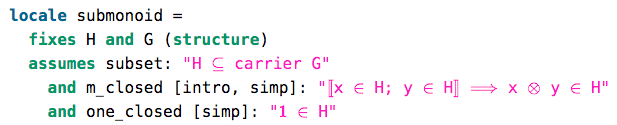
\includegraphics[scale=0.6]{figures/submonoid.png}
%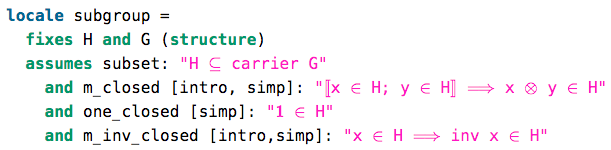
\includegraphics[scale=0.6]{figures/subgroup.png}
\caption{The definition of submonoid and subgroup as defined in Isabelle library. Note how the 
definitions are repeated, although subgroup can be defined as an extension of submonoid.}
\label{fig:isabelle_subalg}
\end{figure*}
The same can also be seen in definitions of products of both theories, shown in Figure 
\ref{fig:isabelle_prod}. 
\begin{figure*}
	\begin{lstlisting}
DirProd :: "_ $\Rightarrow$ _ $\Rightarrow$ ('a $\times$ 'b) monoid" (infixr "$\times \times$" 80) 
  where
	"G $\times \times$ H =
      $\llparenthesis$ carrier = carrier G $\times$ carrier H,
	mult = ($\lambda$(g, h) (g', h'). (g $\otimes\textsubscript{G}$ g', h $\otimes\textsubscript{H}$ h')),
	one = (1$\textsubscript{G}$, 1$\textsubscript{H}$ $\rrparenthesis$"
	\end{lstlisting}
	
	\lstinputlisting[language=Isar, firstline=711, lastline=713]{code/Group.thy}
	\lstinputlisting[language=Isar, firstline=723, lastline=725]{code/Group.thy}
	\caption{The definition of cartesian product of theories in Isabelle library}
	\label{fig:isabelle_prod}
\end{figure*}
Homomorphisms\footnote{defined in \url{HOL/Algebra/Group.thy} and \url{HOL/Algebra/Ring.thy}} 
and quotient algebras\footnote{defined in \url{HOL/Algebra/Coset.thy} and 
\url{HOL/Algebra/QuotRing.thy}} are also 
examples of constructions that are defined in multiple 
places, we show these definitions in Figure \ref{fig:isabelle_hom_quotient}. 
\begin{figure*}
\begin{lstlisting}
definition 
   hom :: "_ $\Rightarrow$ _ $\Rightarrow$ ('a $\Rightarrow$ 'b) set" where 
   "hom G H = 
      {h . h $\in$ carrier G $\rightarrow$ carrier H $\wedge$ 
          ($\forall$ x $\in$ carrier G . $\forall$ y $\in$ carrier G . 
               h (x $\otimes_\textsubscript{G}$ y) = h x $\otimes_\textsubscript{H}$ h y)}
definition 
   ring_hom :: "[('a,'m) ring_scheme,('b,'n) ring_scheme] $\Rightarrow$ 
                                              ('a $\Rightarrow$ 'b) set" 
   where 
   "ring_hom R S = 
      {h . h $\in$ carrier R $\rightarrow$ carrier S $\wedge$ 
        ($\forall$ x y . x $\in$ carrier R $\wedge$ y $\in$ carrier R $\rightarrow$. 
            h (x $\otimes_\textsubscript{R}$ y) = h x $\otimes_\textsubscript{S}$ h y $\wedge$ 
            h (x $\oplus_\textsubscript{R}$ y) = h x $\oplus_\textsubscript{S}$ h y) $\wedge$ 
             h 1$_\textsubscript{R}$ = 1$_\textsubscript{S}$}" 
definition 
    FactGroup :: "[('a,'b) monoid_scheme, 'a set] $\Rightarrow$ ('a set) monoid" 
    (infixl "Mod" 65)
    where FactGroup G H = 
    $\llparenthesis$ carrier = rcosets$_\textsubscript{G}$ H, mult = set_mult G, one = H $\rrparenthesis$
definition 
    FactRing :: "[('a,'b) ring_scheme, 'a set] $\Rightarrow$ ('a set) ring" 
    (infixl "Quot" 65)
    where FactRing R I = 
    $\llparenthesis$ carrier = a_rcosets$_\textsubscript{R}$ I, mult = rcoset_mult R I, 
    one = (I +>$_\textsubscript{R}$ 1$_\textsubscript{R}$), zero = I, add = set_add R $\rrparenthesis$
\end{lstlisting}
%	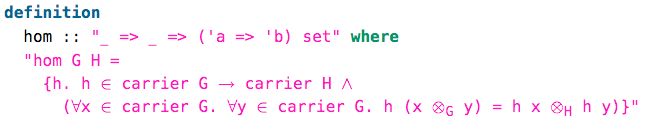
\includegraphics[scale=0.6]{figures/monoid_hom.png}
%	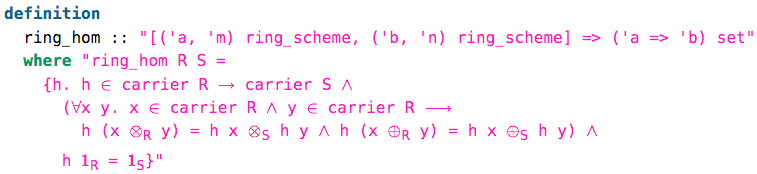
\includegraphics[scale=0.6]{figures/ring_hom.png}
%	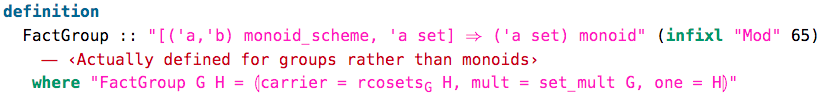
\includegraphics[scale=0.6]{figures/quotient.png}	
%	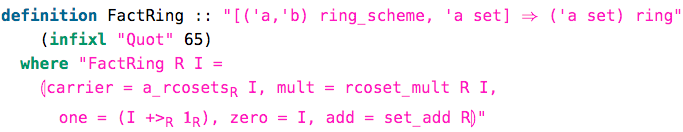
\includegraphics[scale=0.6]{figures/quotient_ring.png}
	\caption{The definition of homomorphisms and quotient algebras in Isabelle library}
	\label{fig:isabelle_hom_quotient}
\end{figure*}
The formalization of these definitions in the library signifies their usefulness. Hand-writing them 
restricts their availability to only a small number of theories. In case users need them for a new theory 
they defined, they have to hand write them. 

\paragraph{Theory presentations are pervasive} Different formal systems have different ways 
for expressing mathematical knowledge. Whether they are called theories, locales, classes, 
modules or records, they all contain the same pieces of information. Figure \ref{ex:monoid} shows 
the representation of \verb|Monoid| theory in $5$ different formal systems. The representation in 
MathScheme (MSL) states the components of \verb|Monoid| as declarations in a theory. 
MMT uses the same approach, but instead of stating the six pieces of \verb|Monoid|, it declares 
\verb|Monoid| as extension of \verb|Semigroup|, So the components of \verb|Monoid| is distributed 
between the two theories. Despite the usefulness of knowing that \verb|Monoid| is an extension of 
\verb|Semigroup|, in some cases the user would really want to see the declarations within the 
theory. MathScheme provides this view of theories, while keeping track of the connection between 
them using the arrows of the graph. 
In Coq, we can see two different representations, both are useful in different ways. The 
\verb|Class| representation expects the function symbols as input to the definition with the axioms 
being the members of the class. The carrier \verb|A| is deduced and need not be passed by the 
user. This allows one to easily define \verb|Monoid|s over the same carrier, operation or unit element, 
which can be beneficial for proving purposes. The \verb|Record| representation does not have the 
same property. Every declaration of monoid is defined as a field in the record. In the case of 
defining two records over the same carrier, the user needs to actually prove they are the same. 
Haskell, as a programming language, does not define axioms or allow proving that instances of the 
class satisfy them. 
The Agda definition have some decorative pieces like \verb|infixl| which specifies that an 
operator is infix and associates left. A monoid can still be defined without those decorative pieces, 
or they can be specified by the user in a declarative manner. 
In all these representations the pieces of information that we need to write the monoid definition is 
the same. Therefore, having one of them should suffice to generate the others. 

We understand that the different representations stem from different design choices of the 
different systems, but this does not deny the fact that they are all representations of the same 
concept of a \verb|Monoid| theory. The possibilities and limitations of moving from one 
representation to another are interesting research points. 
\begin{figure}
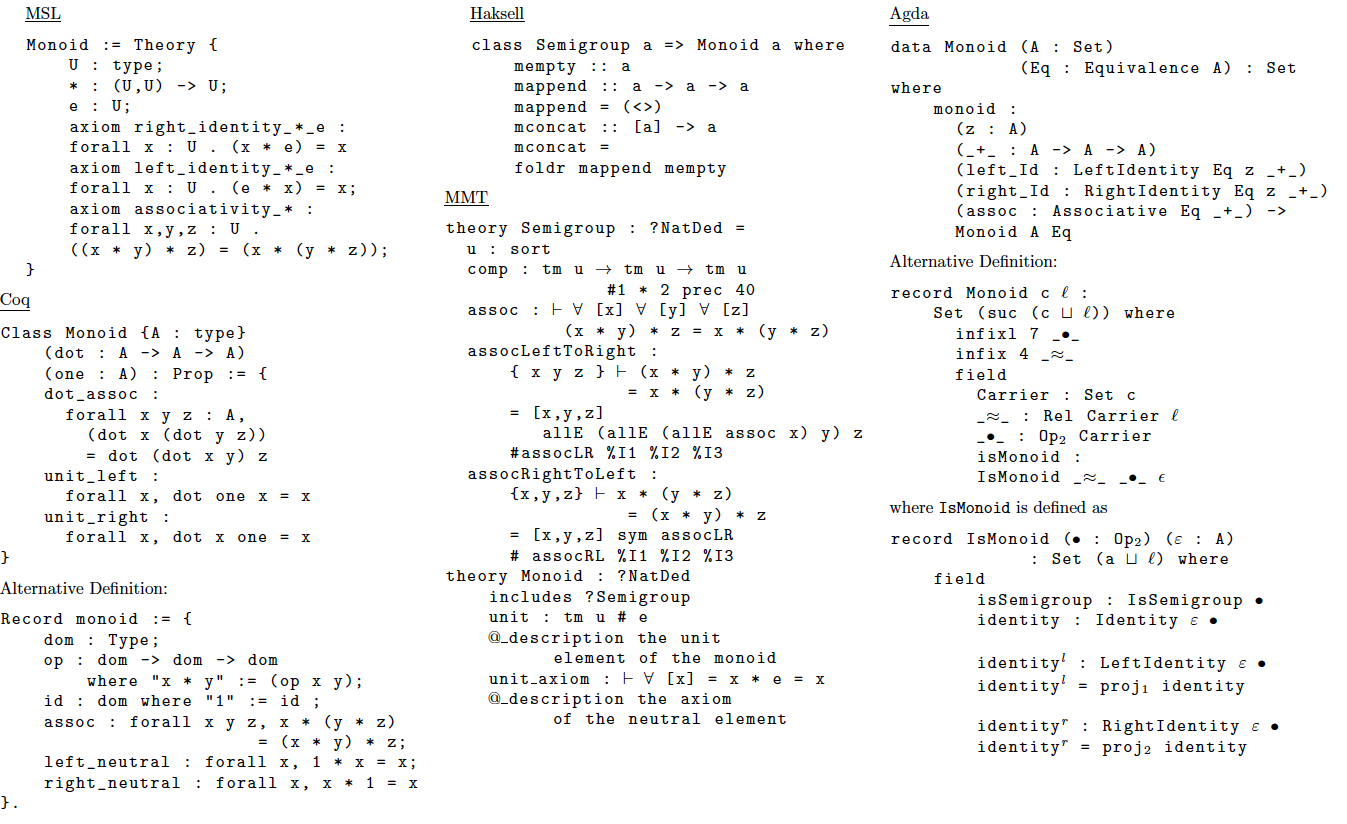
\includegraphics[scale=0.4]{figures/monoid.png}
\caption{The representation of Monoid theory in different formal systems.}
\label{ex:monoid}
\end{figure}

\paragraph{}Our aim in this study is to eliminate the boilerplate associated with defining and using 
theory presentations by automating the generation of related constructions. We imagine the user 
writing an algebraic theory and getting a set of tools customized to her theory that she can directly 
use towards getting her task done. 
%We also believe that having generated this boilerplate code provide the machine with some information about what  concept (eg: signature, language, homomorphism ... etc.) a theory corresponds to, which could be useful in some tasks. 
Our implementation is meant to be generic in terms of the representation language. The toolbox should be able to generate code for different formal systems.
We start by using MathScheme and MMT as data description languages (DDL) of theory presentations, and then generalize to other representations. 

Despite the fact that the algorithms to generate the algebraic structures are the same, non-trivial work 
needs to be done to have generic, re-usable components that generates these structures in different 
representation languages. For example, MSL uses the keyword \verb|axiom| to indicate that an axiom is 
being declared. On the other hand, by using Curry-Howard correspondence, axioms are declared in 
Coq as fields of a class or record definition, in the same way that a function is declared. Therefore, it is 
not easy to distinguish whether a declaration corresponds to a constant, a function or an axiom. Also 
some languages provide special literals to define notations or precedence, while other do not. Dealing 
with these languages as a family and providing re-usable generators is one important aspect of our 
research work. We describe our contribution as:
\begin{itemize}
	\item Evaluating the status of current popular libraries of mathematics, in terms of modularity and 
	reusability.
	\item Compiling a list of constructions that can be automatically generated from the syntax of a theory presentation. 
	\item Building a library of generic algorithms for computing these constructions, given a theory 
	written in DDL, which abstracts over the presentation language. At this point, we only consider 
	theory presentations in their most abstract format as a collection of sorts, function symbols and 
	axioms written in some formal language.  
	\item Implementing generators that can produce these constructions for a specific theory in a 
	specific language, taking into considerations all similarities and differences between different formal 
	systems. We start by the two systems HOL and Agda, but aim to expand the implementation to 
	different systems as time permits.  
\end{itemize}

The expected output of our work is a domain-specific language for developing a library of theories 
structured as theory graphs that minimizes boilerplate, maximizes reuse and generate useful 
information from minimum description. 

In Section \ref{sec:theory_presentations} we describe the class of theory presentations we are 
interested in. We give a brief introduction to MathScheme and MMT, the two frameworks in which 
we conduct our experiments. We present out initial list of constructions that can be automatically 
generated in Section \ref{sec:operations}. We give a summary of related work in Section 
\ref{sec:related_work}. Then we describe the approach we are following in Section 
\ref{sec:approach}. 

